\section{Circle of fifths}

\subsection{What does it say?}

In a previous section the following tables where shown. There was also the term "circle of fifths" and "circle of fourths" mentioned and that this has to do with the fact that there is always one more accidental added ($\sharp$ or $\flat$).

\begin{table}[h]
	\centering
	\begin{minipage}{0.45\textwidth}
		\begin{NiceTabular}{*{16}{P{0.05mm}}}
			\Block{}{} & \Block{1-2}{\large{W}} & & \Block{1-2}{\large{W}} & & \Block{1-2}{\large{H}} & & \Block{1-2}{\large{W}} & & \Block{1-2}{\large{W}} & & \Block{1-2}{\large{W}} & & \Block{1-2}{\large{H}} & & \Block{}{} \\
			\Block{1-2}{\RomanNumeralCaps{1}} & & \Block{1-2}{\RomanNumeral{2}} & & \Block{1-2}{\RomanNumeral{3}} & & \Block{1-2}{\RomanNumeralCaps{4}} & & \Block{1-2}{\RomanNumeralCaps{5}} & & \Block{1-2}{\RomanNumeral{6}} & & \Block{1-2}{\RomanNumeral{7}\textsuperscript{o}} & & \\
			\Block{1-2}{1} & & \Block{1-2}{2} & & \Block{1-2}{3} & & \Block{1-2}{4} & & \Block{1-2}{5} & & \Block{1-2}{6} & & \Block{1-2}{7} & & \Block{1-2}{8} & \\
			\Block{1-2}{F} & & \Block{1-2}{G} & & \Block{1-2}{A} & & \Block{1-2}{B\flat} & & \Block{1-2}{C} & & \Block{1-2}{D} & & \Block{1-2}{E} & & \Block{1-2}{F} & \\
			\Block{1-2}{C} & & \Block{1-2}{D} & & \Block{1-2}{E} & & \Block{1-2}{F} & & \Block{1-2}{G} & & \Block{1-2}{A} & & \Block{1-2}{B} & & \Block{1-2}{C} & \\
			\Block{1-2}{G} & & \Block{1-2}{A} & & \Block{1-2}{B} & & \Block{1-2}{C} & & \Block{1-2}{D} & & \Block{1-2}{E} & & \Block{1-2}{F\sharp} & & \Block{1-2}{G} & \\
			\Block{1-2}{D} & & \Block{1-2}{E} & & \Block{1-2}{F\sharp} & & \Block{1-2}{G} & & \Block{1-2}{A} & & \Block{1-2}{B} & & \Block{1-2}{C\sharp} & & \Block{1-2}{D} & \\
			\Block{1-2}{A} & & \Block{1-2}{B} & & \Block{1-2}{C\sharp} & & \Block{1-2}{D} & & \Block{1-2}{E} & & \Block{1-2}{F\sharp} & & \Block{1-2}{G\sharp} & & \Block{1-2}{A} & \\
			\Block{1-2}{E} & & \Block{1-2}{F\sharp} & & \Block{1-2}{G\sharp} & & \Block{1-2}{A} & & \Block{1-2}{B} & & \Block{1-2}{C\sharp} & & \Block{1-2}{D\sharp} & & \Block{1-2}{E} & \\
			\Block{1-2}{B} & & \Block{1-2}{C\sharp} & & \Block{1-2}{D\sharp} & & \Block{1-2}{E} & & \Block{1-2}{F\sharp} & & \Block{1-2}{G\sharp} & & \Block{1-2}{A\sharp} & & \Block{1-2}{B} & 
		\end{NiceTabular}
		\caption{Major scales of natural notes}
		\label{tab:guitar_major_scales_circle_of_fifths}
	\end{minipage}
	\hfill
	\begin{minipage}{0.45\textwidth}
		\begin{NiceTabular}{*{16}{P{0.05mm}}}
			\Block{}{} & \Block{1-2}{\large{W}} & & \Block{1-2}{\large{H}} & & \Block{1-2}{\large{W}} & & \Block{1-2}{\large{W}} & & \Block{1-2}{\large{H}} & & \Block{1-2}{\large{W}} & & \Block{1-2}{\large{W}} & & \Block{}{} \\
			\Block{1-2}{\RomanNumeral{1}} & & \Block{1-2}{\RomanNumeral{2}\textsuperscript{o}} & & \Block{1-2}{\RomanNumeralCaps{3}} & & \Block{1-2}{\RomanNumeral{4}} & & \Block{1-2}{\RomanNumeral{5}} & & \Block{1-2}{\RomanNumeralCaps{6}} & & \Block{1-2}{\RomanNumeralCaps{7}} & & \\
			\Block{1-2}{1} & & \Block{1-2}{2} & & \Block{1-2}{3$\flat$} & & \Block{1-2}{4} & & \Block{1-2}{5} & & \Block{1-2}{6$\flat$} & & \Block{1-2}{7$\flat$} & & \Block{1-2}{8} & \\
			\Block{1-2}{B} & & \Block{1-2}{C\sharp} & & \Block{1-2}{D} & & \Block{1-2}{E} & & \Block{1-2}{F\sharp} & & \Block{1-2}{G} & & \Block{1-2}{A} & & \Block{1-2}{B} & \\
			\Block{1-2}{E} & & \Block{1-2}{F\sharp} & & \Block{1-2}{G} & & \Block{1-2}{A} & & \Block{1-2}{B} & & \Block{1-2}{C} & & \Block{1-2}{D} & & \Block{1-2}{E} & \\
			\Block{1-2}{A} & & \Block{1-2}{B} & & \Block{1-2}{C} & & \Block{1-2}{D} & & \Block{1-2}{E} & & \Block{1-2}{F} & & \Block{1-2}{G} & & \Block{1-2}{A} & \\
			\Block{1-2}{D} & & \Block{1-2}{E} & & \Block{1-2}{F} & & \Block{1-2}{G} & & \Block{1-2}{A} & & \Block{1-2}{B\flat} & & \Block{1-2}{C} & & \Block{1-2}{D} & \\
			\Block{1-2}{G} & & \Block{1-2}{A} & & \Block{1-2}{B\flat} & & \Block{1-2}{C} & & \Block{1-2}{D} & & \Block{1-2}{E\flat} & & \Block{1-2}{F} & & \Block{1-2}{G} & \\
			\Block{1-2}{C} & & \Block{1-2}{D} & & \Block{1-2}{E\flat} & & \Block{1-2}{F} & & \Block{1-2}{G} & & \Block{1-2}{A\flat} & & \Block{1-2}{B\flat} & & \Block{1-2}{C} & \\
			\Block{1-2}{F} & & \Block{1-2}{G} & & \Block{1-2}{A\flat} & & \Block{1-2}{B\flat} & & \Block{1-2}{C} & & \Block{1-2}{D\flat} & & \Block{1-2}{E\flat} & & \Block{1-2}{F} & 
		\end{NiceTabular}
		\caption{Minor scales of natural notes}
		\label{tab:guitar_minor_scales_circle_of_fifths}
	\end{minipage}
\end{table}

Take a look at the circle in \autoref{fig:guitar_circle_of_fifths}. Things to note:

\begin{figure}[h]
	\centering
	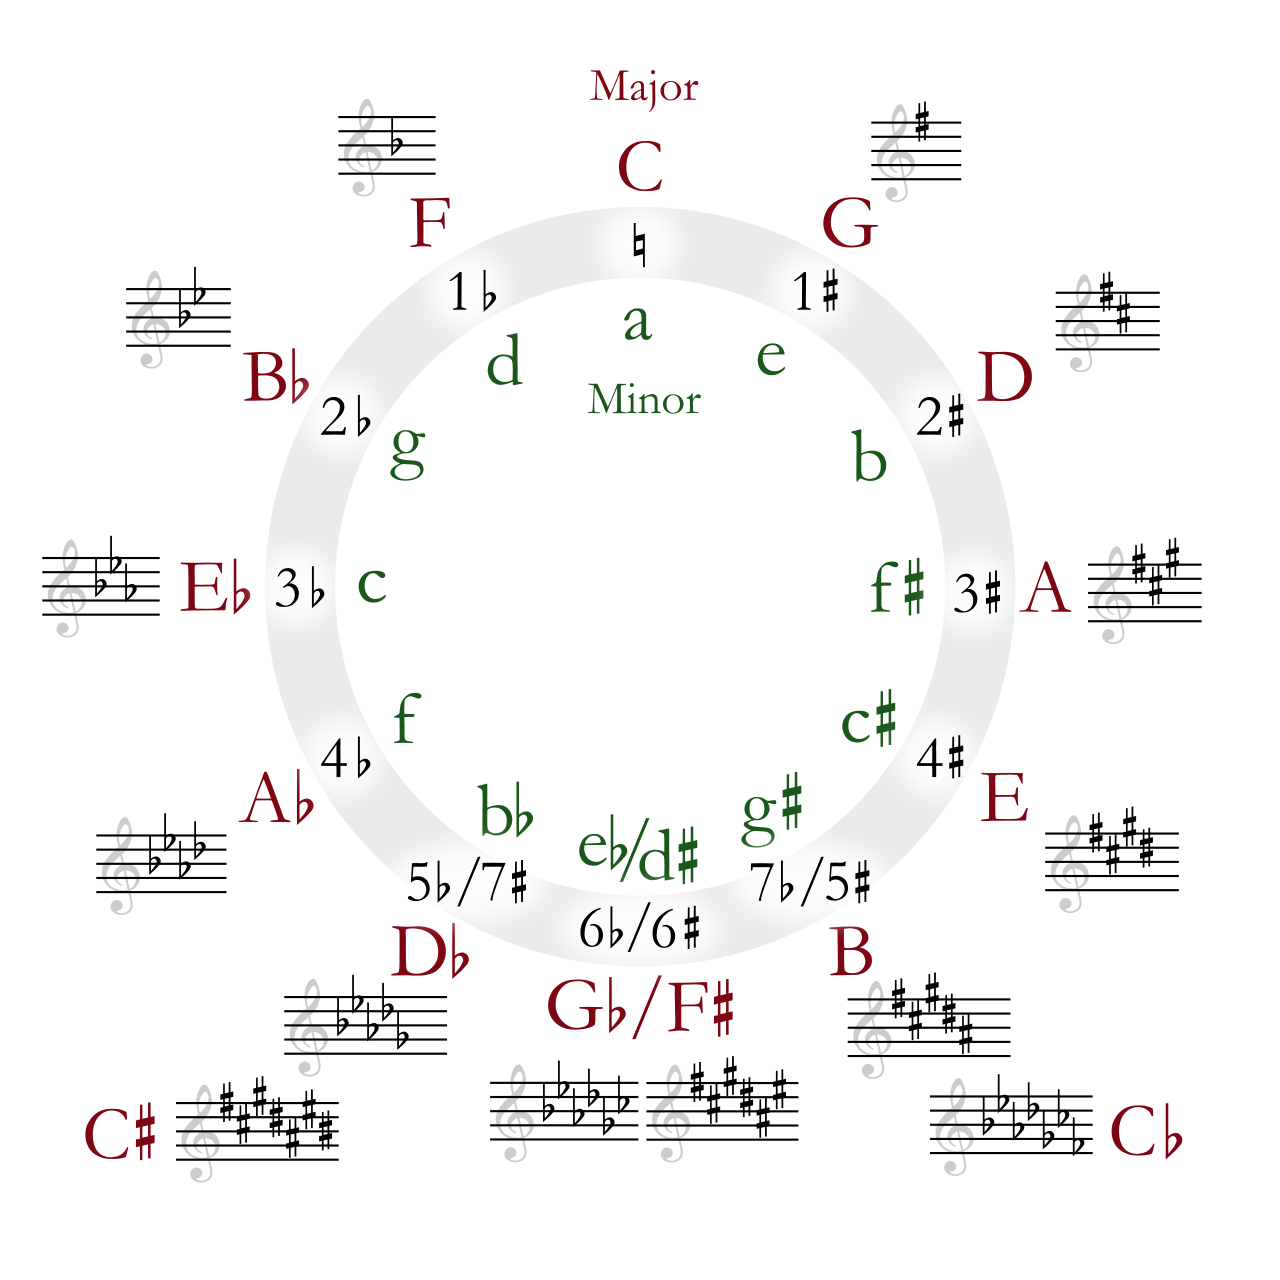
\includegraphics[width=0.55\textwidth]{../../Images/Circle_of_fifths_deluxe_4.svg.png}
	\caption{Circle of fifths \cite{CircleOfFifthsImageWikipedia}}
	\label{fig:guitar_circle_of_fifths}
\end{figure}

\begin{itemize}
	\item \textbf{Going clockwise:} Each note on the right of a note, is the \textbf{5th degree} in the major scale of the note. We went \textbf{up a perfect 5th interval}.
	\item \textbf{Going counterclockwise:} Each note on the left of a note, is the \textbf{4th degree} in the major scale of the note. We went \textbf{down a perfect 5th interval}. To see this, look at \autoref{tab:guitar_major_scales_circle_of_fifths}, start at the 8th degree and count the number of half-steps when you go back to the 4th degree. This is 7 half-steps. Now look at \autoref{tab:guitar_intervals_in_octave} and see that 7 half-steps (semitones) is a perfect 5th interval.
\end{itemize}

\begin{itemize}
	\item \textbf{Going clockwise:} With each new 'step' a $\sharp$ is added. 
	\item \textbf{Going counterclockwise:} With each new 'step' a $\flat$ is added.
\end{itemize}

The $\sharp$ and $\flat$ that are added both follow the same mnemonic but one of them is reversed:

\begin{table}[h]
	\centering
	\begin{NiceTabular}{r | l l l l l l l}
		Clockwise ($\sharp$) & \textbf{F}ather & \textbf{C}harles & \textbf{G}oes & \textbf{D}own & \textbf{A}nd & \textbf{E}nds & \textbf{B}attle \\
		Counterclockwise ($\flat$) & \textbf{B}attle & \textbf{E}nds & \textbf{A}nd & \textbf{D}own & \textbf{G}oes & \textbf{C}harles & \textbf{F}ather \\
	\end{NiceTabular}
\end{table}

Note how the sharps and flats are separated by a perfect 5th as well.

\newpage

\subsection{Using the circle of fifths}

\subsubsection{Relative minor/major scales}

If you compare the notes in the C major and A minor scales, you see that they have the same notes. This means that A minor is the \textbf{relative minor} of C major. And vice verse, C major is the \textbf{relative major} of A minor. The inner circle in the circle of fifths (the minor circle), show the relative minor scales to the outer (major) circle (and vice verse).

So you can quickly see that the relative minor of E$\flat$ major is C minor, and that the relative major key of B minor is D major.

\subsubsection{Quickly showing chords in a scale}

In the beginning of this chapter you have already that there are major, minor, and diminished chords in a scale and how to identify these. These chords where identified with roman numerals.

\underline{Chords in the major scale}

We start at a note on the major circle.

It was already said that the note on the right is the 5th degree of a scale, the note on the left is the 4th degree of a scale.

The 6th degree in the major scale is the relative minor. If you go a perfect 5th (7 semitones) up from the 6th degree in the major scale, you end up at the 3rd degree. If you go down a perfect 5th, you end up at the 2nd degree.

The remaining chord is the diminished chord. This can be found by going up a perfect 5th from the 3rd degree (one step to the right).

\underline{Chords in the minor scale}

We start at a note on the minor scale.

The perfect 4th and perfect 5th interval are in both the major and minor scale. Meaning that on the right we have the 5th degree and on the left we have the 4th degree in the minor scale (by going up and down a perfect 5th respectively).

The relative major is the 3rd degree. Going up a perfect 5th from the 3rd degree in the minor scale lands on the 7th degree. Going down a perfect 5th in the minor scale lands on the 6th degree.

To get the remaining diminished chord you go up a perfect 5th from the 5th degree in the minor scale.

\begin{figure}[h]
	\centering
	\begin{subfigure}{0.47\textwidth}
		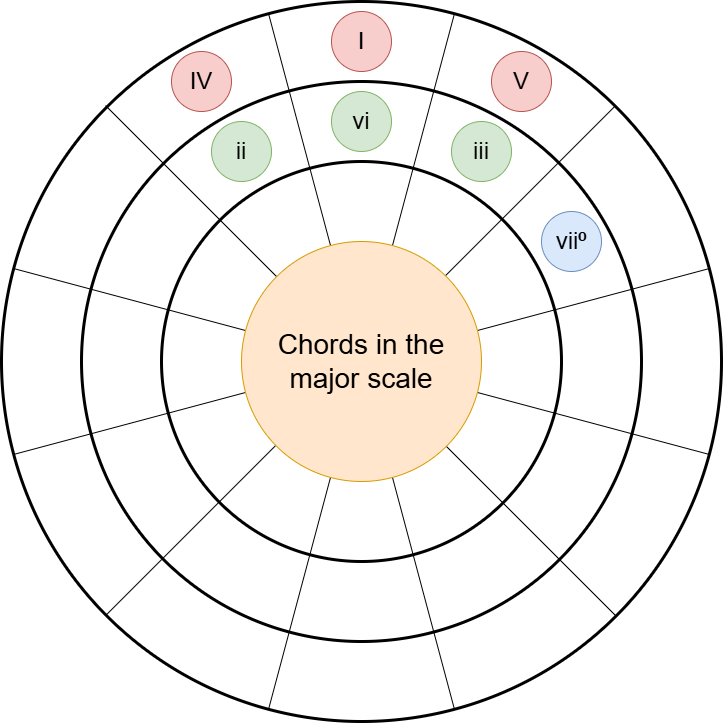
\includegraphics[width=\textwidth]{../../Images/CircleOfFifthsChordsInTheMajorScale.png}
		\caption{Circle of fifths: major scale chords}
		\label{fig:circle_of_fifths_major_scale_chords}
	\end{subfigure}
	\hfill
	\begin{subfigure}{0.47\textwidth}
		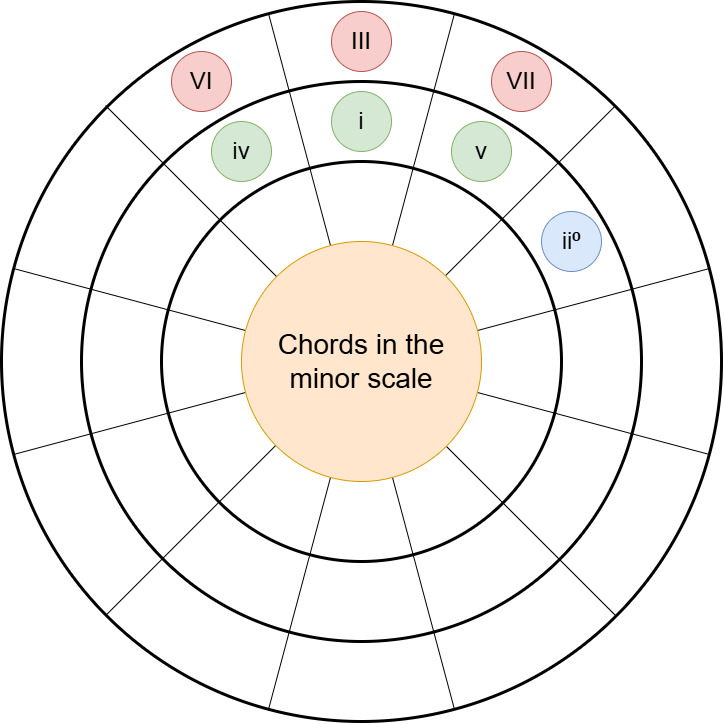
\includegraphics[width=\textwidth]{../../Images/CircleOfFifthsChordsInTheMinorScale.png}
		\caption{Circle of fifths: minor scale chords}
		\label{fig:circle_of_fifths_minor_scale_chords}
	\end{subfigure}
	\caption{Rotatable chord degrees in the circle of fifths}
\end{figure}

\newpage

\subsubsection{Starting point for identifying the key of sheet music}

If you see 3 $\sharp$s at the beginning on the sheet music, the song will (mostly) use notes from the A major key (which are the same notes of F$\sharp$ minor key). To determine if the song is major, minor, or any other mode (more about this in \autoref{sec:modes}) you need more context of the notes in the song.

\subsubsection{Seeing which keys to change and modulate to}

When you go through the circle there is always one note that is different (an added/removed $\sharp$/$\flat$).

So if you want to modulate to a new key, you can use the circle of fifth to determine how 'rapid' you want to change to be. Or to see through which keys you can go to reach the 'final' key.

\underline{Example of abrupt key change}

In "Livin' On A Prayer" from "Bon Jovi" there is a key change in the outro-chorus. It goes from E minor to G minor. Both use the same chord progression.

\begin{table}[h]
	\centering
	\begin{NiceTabular}{|l|c|c|c|c|c|c|}
		\hline
		\backslashbox{Key}{Chord} & \RomanNumeral{1} & \RomanNumeralCaps{6} & \RomanNumeralCaps{7} & \RomanNumeralCaps{3} & \RomanNumeralCaps{6} & \RomanNumeralCaps{7} \\
		\hline
		E minor & Em & C & D & G & C & D \\
		\hline
		G minor & Gm & E$\flat$ & F & B$\flat$ & E$\flat$ & F \\
		\hline
	\end{NiceTabular}
\end{table}


\begin{song}[verse/numbered, align-chords=l]{title={Livin' On A Prayer - Bon Jovi}, music={Bon Jovi}}
	\begin{chorus}
		^{Em}Oh, ^{C} we're ^{D}halfway there, ^{G}woah ^{C}oh, ^{D}livin' on a prayer. \\
		^{Em}Take my ^{C}hand, we'll ^{D}make it I swear \\
		^{G}Woah ^{C}oh, ^{D}livin' on a prayer. \\
	\end{chorus}
	
	\begin{outro-chorus}
		^*{Gm}Woooo ^{Eb}oo, we're ^{F}halfway there, ^{Bb}Woah ^{Eb}oh, ^{F}livin' on a prayer. \\
		^{Gm}Take my ^{Eb}hand and we'll ^{F}make it I swear \\
		^{Bb}Woah ^{Eb}oh, ^{F}livin' on a prayer. \\
	\end{outro-chorus}
\end{song}

Looking at \autoref{fig:guitar_circle_of_fifths}, you see that G minor is 3 steps to the left of E minor. Meaning there are quite some different notes between both scales.

Also if you look at the scale of E minor (in \autoref{tab:guitar_minor_scales_circle_of_fifths}) then you see that G is the 3rd degree in the scale (a minor 3rd interval). Meaning that the G is an important note that makes the E minor scale, minor.

\newpage

\underline{Example of pivot chord/note}

In "We Are The Champions" from "Queen" an example of a pivot chords/note can be seen. This song changes not only from key, but also from mode. It goes from C minor (during the verses) to F major (during the chorus).

\autoref{fig:circle_of_fith_overlap_c_minor_f_major} shows that there are two overlapping chords (B$\flat$, G minor) and five overlapping notes (B$\flat$, C, D, F, G) in these two keys. Note that no D minor chord was mentioned as overlapping chord. This is because in the C minor key the \textit{d} is a diminished chord, while in the F major key \textit{d} is a minor chord. In "We Are The Champions", B$\flat$ is used as the pivot chord/note to connect the C minor to the F major keys.

Additionally, at the end of the verse, a C7 chord is played which is in the F major scale but not in the C minor scale. The Cm chord contains \textit{C, E$\flat$, G}. The C7 chord contains \textit{C, E, G, B$\flat$}. The only note in the C7 that makes it F major scale specific is the E note.

\begin{figure}[h]
	\centering
	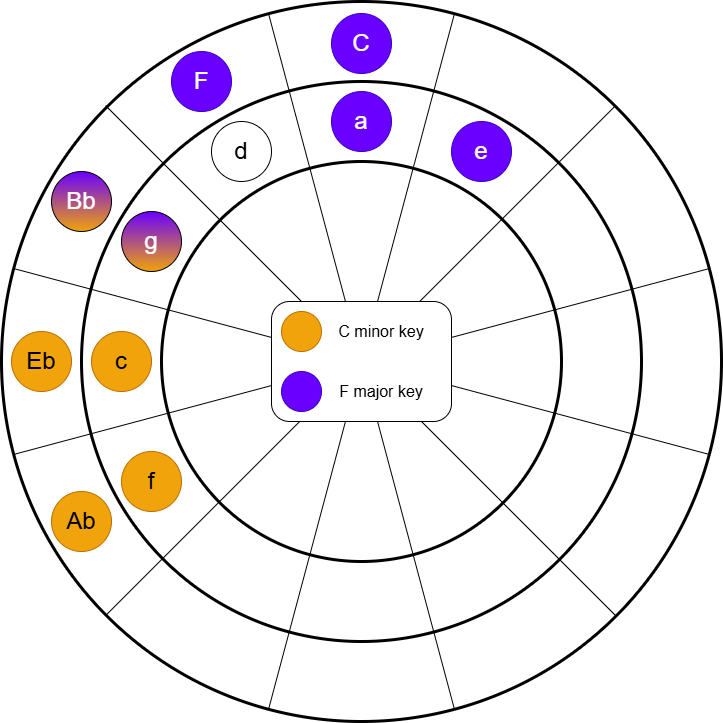
\includegraphics[width=0.45\textwidth]{../../Images/CircleOfFifthsCminorFmajor.png}
	\caption{Showing the overlap of the chords in C minor (orange) and F major (purple)}.
	\label{fig:circle_of_fith_overlap_c_minor_f_major}
\end{figure}

\infobox{Some of these chord names are not discussed yet. This will be described in the next chapter. However, to already play along, see the chord shapes on the next page (\autoref{fig:queen_we_are_the_champions_key_change_chords}).}

\begin{song}[align-chords=l]{title={We Are The Champions - Queen}, music={Queen}} \label{song:we_are_the_champions_queen}
	\begin{verse}
		I've had my ^{Eb}share of sand ^{Bb}kicked in my ^{Cm}face \\
		But ^{F7}I've come ^{Bb}through \\
		And I mean to go ^{Ab/Bb}on, and ^{Bbm7(b5)}on, and ^{Bb7}on, and ^{C7}on \\
	\end{verse}
	
	\begin{chorus}
		^{F}We are the ^{Am}champions, my ^{Dm}friends ^{Bb} ^{C7} \\
		And ^{F}we'll keep on ^{Am}fighting till the ^{Bb}end ^{F#dim7} \\
		^{Gm}We are the ^{C7/G}champions, ^{Bbm}we are the ^{Edim7}champions \\
		^{F}No time for ^{Gm}losers 'cause ^{Ab}we are the ^{Bb}champions ^{C7sus4} \\
		Of the ^{Fm}world ^{Gm7}
 	\end{chorus}
\end{song}

\newpage

\begin{figure}[h]
	\centering
	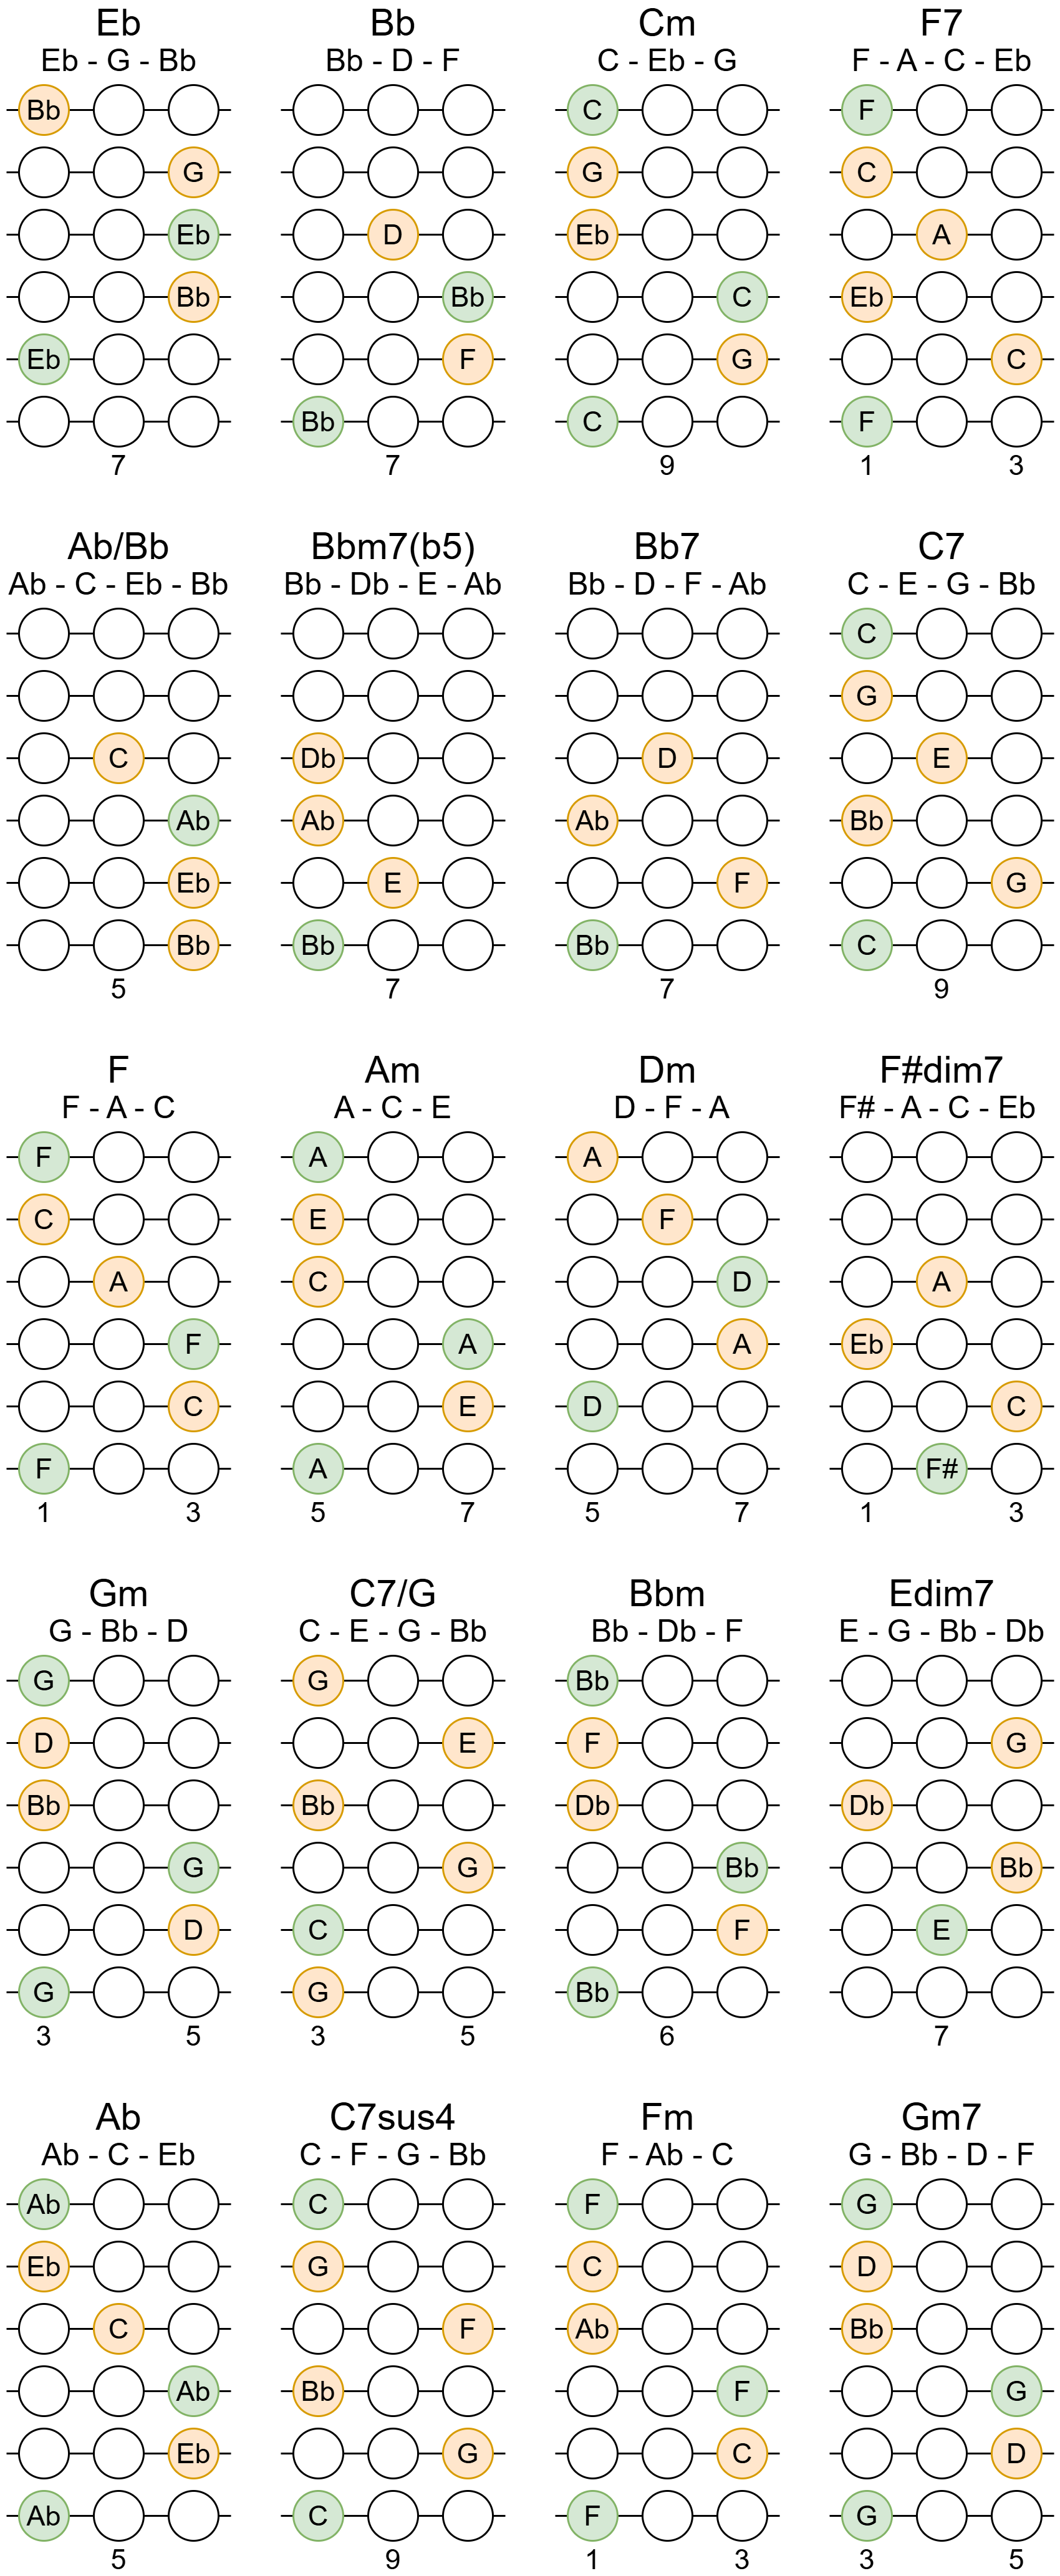
\includegraphics[width=0.65\textwidth]{../../Images/WeAreTheChampionsQueenKeyChangeChords.png}
	\caption{Some of the chords in "We Are The Champions" - Queen}.
	\label{fig:queen_we_are_the_champions_key_change_chords}
\end{figure}


\newpage